\section{CMOS-Logik}

\begin{itemize}
    \item Entweder leitender Pfad nach $V_{SS}$ (NMOS) oder $V_{DD}$ (PMOS)
    \item Kein statischer Stromverbrauch
    \item Langsamer als Bipolar
    \item Symmetrische Schaltschwellen bei ca. $\frac{V_{DD}}{2}$ (Übertrgaungskennlinie)
    \item Output-Level $V_{ol}$, $V_{oh}$ näher bei Speisung als Input Level $V_{il}$, $V_{ih}$ \textrightarrow\ mehr Marge
    \item Höhere Speisespannung \textrightarrow\ weniger propagation delay
    \item Nicht geeignet zur Datenübertragung über längere Strecken (kein $50 \, \ohm$ Abschluss)
\end{itemize}


\subsection{Grundgatter in CMOS-Logik}

\begin{minipage}[t]{0.32\columnwidth}
    \begin{center}
        \textbf{Inverter} \\
        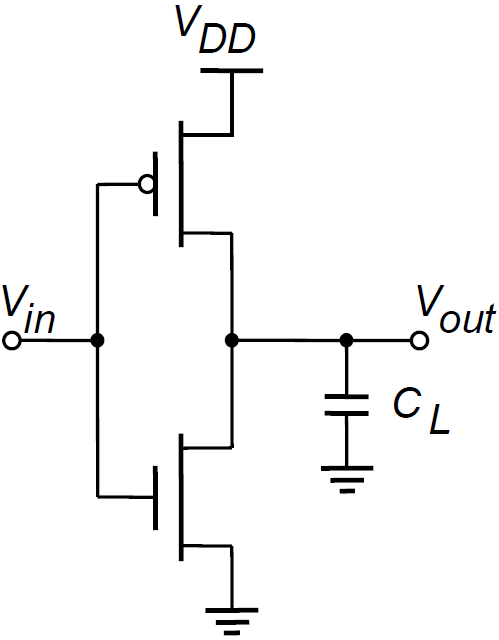
\includegraphics[width=\columnwidth]{images/cmos_inverter.png}
    \end{center}
\end{minipage}
\hfill
\begin{minipage}[t]{0.27\columnwidth}
    \begin{center}
        \textbf{NAND-Gate} \\
        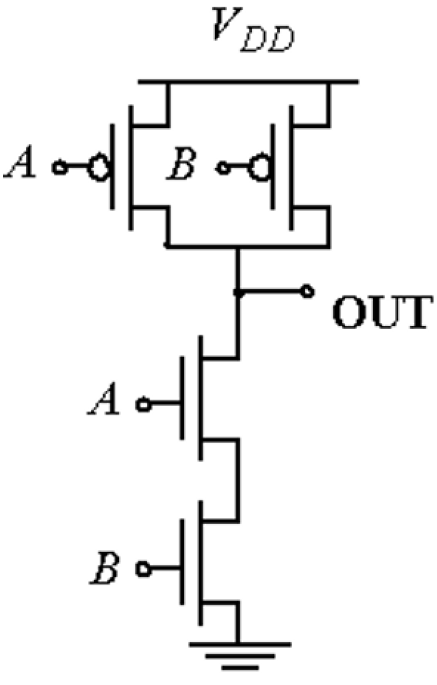
\includegraphics[width=\columnwidth]{images/cmos_nand_2.png}
    \end{center}
\end{minipage}
\hfill
\begin{minipage}[t]{0.38\columnwidth}
    \begin{center}
        \textbf{NOR-Gate} \\
        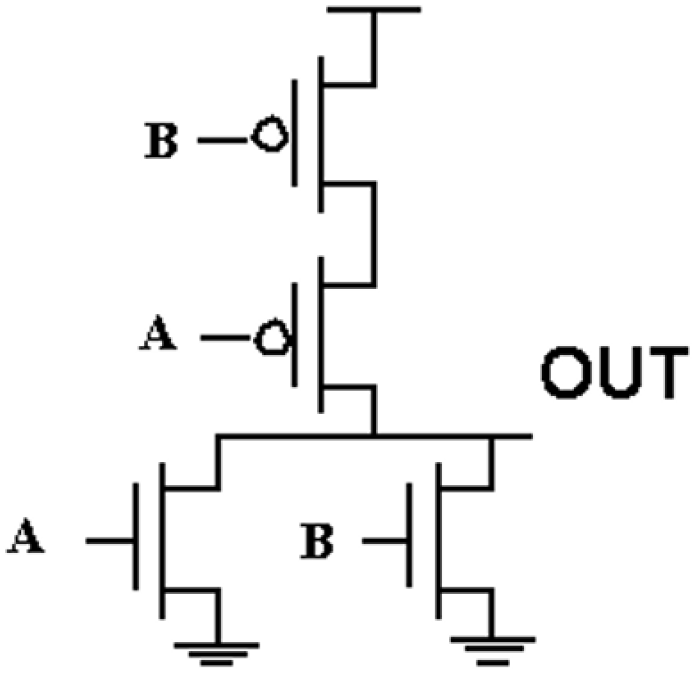
\includegraphics[width=\columnwidth]{images/cmos_nor.png}
    \end{center}
\end{minipage}


\subsection{Dualität NMOS - PMOS}

\begin{minipage}[c]{0.45\columnwidth}
    \begin{center}
        \textbf{PMOS} \\
        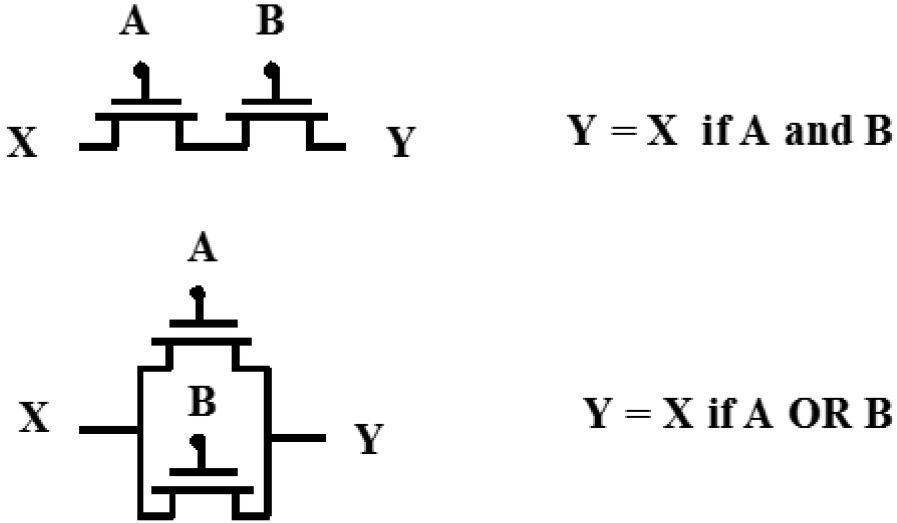
\includegraphics[width=\columnwidth]{images/nmos_dualitaet.png}
    \end{center}
\end{minipage}
\hfill
\begin{minipage}[c]{0.45\columnwidth}
    \begin{center}
        \textbf{NMOS} \\
        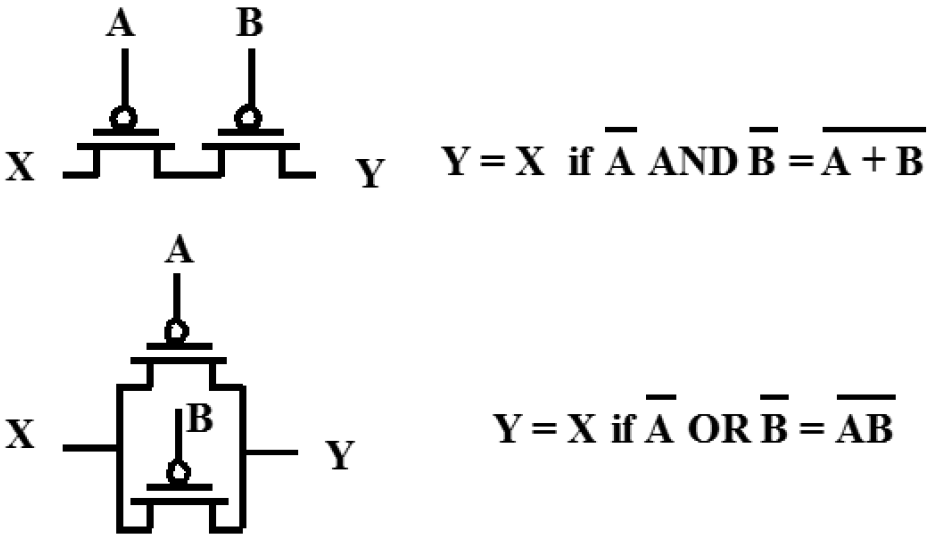
\includegraphics[width=\columnwidth]{images/pmos_dualitaet.png}
    \end{center}
\end{minipage}


\subsection{Verlustleistung bei CMOS-Logik}

\begin{minipage}[c]{0.48\columnwidth}
    $$ \boxed{ P_V = C \cdot V_{CC}^2 \cdot f} $$
\end{minipage}
\hfill
\begin{minipage}[c]{0.48\columnwidth}
    \begin{tabular}{ll}
        $C$ & Kapazität (aus Datenblatt) \\
        $f$ & Frequenz 
    \end{tabular}
\end{minipage}


\subsection{Verzögerungszeit}

\begin{minipage}[t]{0.48\columnwidth}
    \textbf{Linearer Bereich}
    $$ \boxed{t_{pHL} = 0.69 \cdot R_{on} \cdot C_L} $$
    \textrightarrow\ Exponentielle Entladung! 
\end{minipage}
\hfill
\begin{minipage}[t]{0.48\columnwidth}
    \textbf{Sättigung (Stromquellen-Bereich)}
    $$ \boxed{t_{pHL} = \frac{C_L \cdot \frac{V_{swing}}{2}}{I_{sat}} \approx \frac{C_L}{k_n \cdot V_{DD}} }$$
    \textrightarrow\ Lineare Entladung!
\end{minipage}


% TODO: Kennlinien / Charakteristik CMOS-Technologie...?
% \section{CMOS  vs. TTL Logikpegel}
% 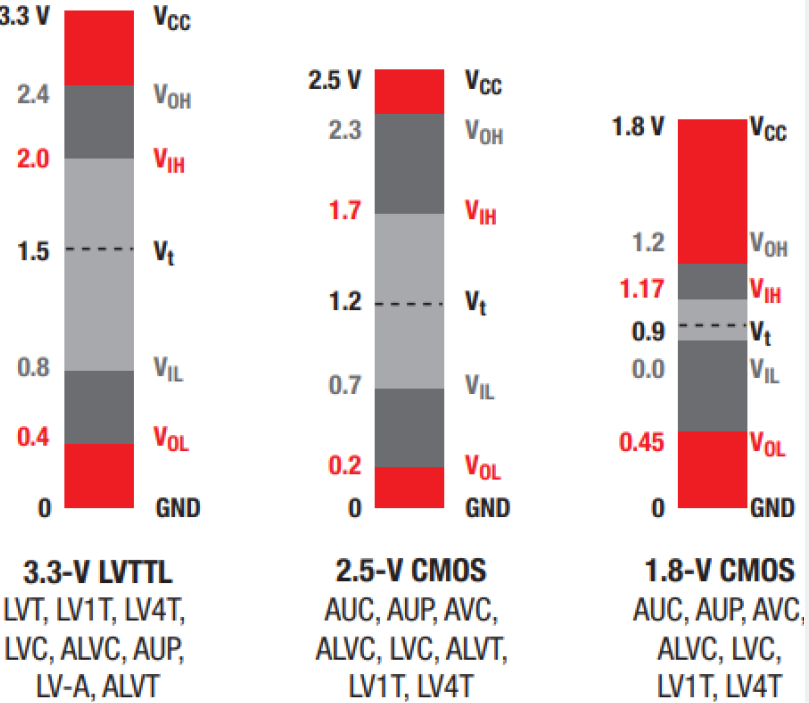
\includegraphics[width=0.75\columnwidth]{images/logik_pegel.png}